\documentclass[a4paper]{article}
\usepackage{amsmath,amssymb,mathtools,bm,etoolbox}

\begin{document}
\title{Writing Exercise}
\author{Bochen Wang, Tianyuan Liu}
\maketitle
\section*{Exercise 14.2}
\subsection*{1}
The log-likelihood of data \\
\begin{eqnarray*}
	\prod\limits_{i=1}^{N}g(x_i) &=& \prod\limits_{i=1}^{N}(\sum\limits_{k=1}^{K}\pi_k g_k(x_i)) \\
	l(\theta;Z) &=& \log {\prod\limits_{i=1}^{N}g(x_i)} \\
	&=& \sum\limits_{i=1}^{N}\log (\sum\limits_{k=1}^{K}\pi_k g_k(x_i)) \\
\end{eqnarray*} 

\subsection*{2}
Maximize the log-likelihood above using EM algorithm \\
Pretend we know the value of latent variable $ \Delta $ for each point:\\
\begin{align*}
	l(\theta;Z,\Delta) = \sum \limits_{i=1}^{N} \Delta_{k,i} \log g_k(x_i;\mu_k,\sigma_k^2) + \sum \limits_{i=1}^{N} \Delta_{k,i} \log \pi_k  \\
\end{align*}
E-step \\
For k = 1 to K, i = 1 to N\\
\begin{eqnarray*}
	T_{k,i} &=& E(\Delta_{k,i}|\theta,Z) \\
	 &=& \frac{\pi_k g_k(x_i;\mu_k,\sigma_k^2)}{\sum\limits_{k=1}^{K} \pi_k g_k(x_i;\mu_k,\sigma_k^2)} 
\end{eqnarray*}
M-step \\
For k = 1 to K\\
\begin{center}	
	\mu_k = \frac{\sum \limits_{i=1}^{N} T_{k,i} x_i}{\sum\limits_{i=1}^{N} T_{k,i}} \\
	\sigma^2_k = \frac{\sum \limits_{i=1}^{N} T_{k,i} (x_i-\mu_k)}{\sum \limits_{i=1}^{N} T_{k,i}}\\
	\pi_k = \frac {\sum \limits _{i=1}^{N} T_{k,i}}{N} \\	
\end{center}
\subsection*{3}
\begin{center}
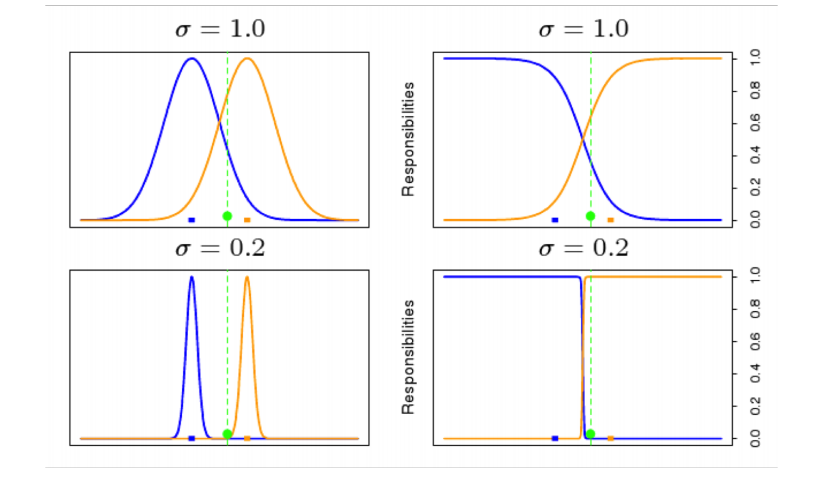
\includegraphics[scale = 0.6]{responsbility}
\end{center}
As the figure above shows, when $ \sigma \rightarrow 0 $, the responsibility curve is very steep. There is almost no soft assign interval. So the data point will no longer spreads to each mode, it will be assign to a specific mode. So that when $ \sigma \rightarrow 0 $, EM algorithm turns into K-Means.


\section*{Exercise 14.8}

For the Procrustes transformation we want to evaluate 
\begin{align*}
	\underset{\mu,R}{\DeclareMathOperator{\argmin}{arg\,min}} \lVert X_2-(X_1 R + \bm{1}\mu^T) \rVert _F
\end{align*}
$R$ is the rotation matrix, $\mu$ is the translation vector. \\
It has the same solution as
\begin{align*}
	\underset{\mu,R}{\DeclareMathOperator{\argmin}{arg\,min}} \lVert X_2-(X_1 R + \bm{1}\mu^T) \rVert _F ^2 \\
	\because \lVert X \rVert _F ^2 = trace(X^T X) \\
\end{align*}
So the function we want to evaluate can be written as 
\begin{align*}
	\underset{\mu,R}{\DeclareMathOperator{\argmin}{arg\,min}} [trace((X_2-X_1 R - \bm{1}\mu^T)^T(X_2-X_1 R - \bm{1}\mu^T))]
\end{align*}

\begin{eqnarray*}
	(X_2-X_1 R - \bm{1}\mu^T)^T(X_2-X_1 R - \bm{1}\mu^T) &=& ((X_2-X_1 R)^T-\mu \bm{1}^T)((X_2-X_1 R)-\bm{1}\mu^T)\\
	&=& (X_2-X_1 R)^T(X_2-X_1 R) \\
	&-& (X_2-X_1 R)^T \bm{1}\mu^T-\mu \bm{1}^T(X_2-X_1 R)\\
	&+& \mu \bm{1}^T \bm{1} \mu^T\\
	\because \bm{1}^T \bm{1} &=& N\\
	\bm{1}^TX_1 &=& N \bar{x}_1^T\\
	\bm{1}^TX_2 &=& N \bar{x}_2^T\\	
\end{eqnarray*}
Minimize the trace above by taking the $ \mu $ derivative and set the derivative to zero.
\begin{eqnarray*}
	-2(X_2-X_1 R)^T\bm{1} + 2N\mu &=& 0 \\
	\mu &=& \frac{1}{N} (X_2^T-R^T X_1^T)\bm{1} \\
	&=& \bar{x}_2-R^T\bar{x}_1 
\end{eqnarray*}
With the $\mu$ we calculate, we can simplify the trace.
\begin{eqnarray*}
	X_2-X_1 R- \bm{1}\mu^T &=& X_2 - X_1 R - \bm{1}(\bar{x}_2^T-\bar{x}_1^T R) \\
	&=& X_2-\bm{1}\bar{x}_2^T-(X_1-\bm{1}\bar{x}_1^T)R \\
	&=& \tilde{X}_2-\tilde{X}_1 R\\
\end{eqnarray*}
Original problem transform into
\begin{align*}
	\underset{R}{\DeclareMathOperator{\argmin}{arg\,min}} [trace((\tilde{X}_2-\tilde{X}_1 R)^T(\tilde{X}_2-\tilde{X}_1 R))]
\end{align*}
To solve this, we have $RR^T=R^TR=I$, so we define a Lagrangean function as below.
\begin{eqnarray*}
	\text{Let } E &=& \tilde{X}_2-\tilde{X}_1 R \\
	F &=& trace(E^TE) + trace(L(R^TR-I)) \\
	\frac{\partial{F}}{\partial{R}} &=&  -2\tilde{X}_1^T\tilde{X}_2+2\tilde{X}_1^T\tilde{X}_1 R + R(L+L^T) \\
	\text{Let } \frac{\partial{F}}{\partial{R}} &=& 0 \\
\end{eqnarray*}
We get the equation below.
\begin{eqnarray*}
	\frac{L+L^T}{2} &=& -R^T \tilde{X}_1^T \tilde{X}_2 + R^T \tilde{X}_1^T \tilde{X}_1 R\\
\end{eqnarray*}
Because $ \frac{L+L^T}{2} $ is symmetric and $ R^T \tilde{X}_1^T \tilde{X}_1 R $ is symmetric too, $ R^T \tilde{X}_1^T \tilde{X}_2 $ must be symmetric.
\begin{eqnarray*}
	\text{Let } S &=& \tilde{X}_1^T \tilde{X}_2 \\
	\text{Has } R^T S &=& S^T R \\
	S &=& R S^T R \\
	\text{Also } S^T &=& R^T S R^T \\
	S S^T &=& R S^T S R^T \\
\end{eqnarray*}
Implement the SVD on $ S $.
\begin{eqnarray*}
	S &=& UDV^T \\
	S S^T &=& UDV^TVDU^T \\
	&=& U D^2 U^T \\
	S^T S &=& VDU^TUDV^T\\
	&=& VD^2V^T\\
	\because SS^T &=& R S^T S R^T\\
	\therefore UD^2U^T &=& R VD^2V^T R^T \\
	\therefore R &=& UV^T \\
\end{eqnarray*}
When we add the scaling parameter. We want to evaluate
\begin{align*}
	\underset{\beta,R}{\DeclareMathOperator{\argmin}{arg\,min}} \lVert X_2- \beta X_1 R \rVert _F
\end{align*}
Familiar with the result above, we got $ R = UV^T $. \\
Now we need to get $\beta$.
\begin{eqnarray*}	
	\frac{\partial{F}}{\partial{\beta}} &=& 2 \beta \text{ trace}(R^T X_1^T X_1 R) - 2 \text{ trace}(X_2^T X_1 R) \\
	\text{Let } \frac{\partial{F}}{\partial{\beta}} &=& 0\\
	\beta &=& \frac{trace(X_2^T X_1 R)}{trace(R^T X_1^T X_1 R)} \\
	&=& \frac{trace(X_2^T X_1 R)}{trace(X_1^T X_1 R R^T)} \\
	&=& \frac{trace(R^T X_1^T X_2)}{trace(X_1^T X_1)} \\
	&=& \frac{trace(VU^TUDV^T)}{\lVert X_1 \rVert _F^2} \\
	&=& \frac{trace(U^TUDV^TV)}{\lVert X_1 \rVert _F^2} \\
	&=& \frac{trace(D)}{\lVert X_1 \rVert _F^2}\\
\end{eqnarray*}

\section*{Exercise 14.11}
In the multiscaling problem, we have the square distance matrix and we want to reconstruct the observation matrix $X$. In classical multiscaling problem we get the centered inner product matrix, and we want to reconstruct observation matrix $X$. \\
Let $X$ denotes the original observation data matrix with $N \times p $ dimension. \\
Let $X_c$ denotes the centered data matrix with subtracted column means. \\
We have 
\begin{eqnarray*}
	X_c &=& (I-\frac{\bm{1}\bm{1}^T}{n})X \\
	\text{Let } S &=& X_cX_c^T\\
\end{eqnarray*}
So $S$ is the centered inner product matrix with elements $<x_i-\tilde{x},x_j-\tilde{x}>$.\\
Now we need to use square distance matrix $d^2$ to get $S$.
\begin{eqnarray*}
	d_{i,j}^2 &=& \lVert x_i - x_j \rVert ^2 \\
	&=& \lVert (x_i - \tilde{x}) - (x_j - \tilde{x}) \rVert ^2 \\
	&=& \lVert x_i - \tilde{x} \rVert ^2 + \lVert x_j - \tilde{x} \rVert ^2 - 2<x_i-\tilde{x},x_j-\tilde{x}>\\
	&=& \lVert x_i - \tilde{x} \rVert ^2 + \lVert x_j - \tilde{x} \rVert ^2 - 2 S_{i,j} \\
	\therefore S &=& -\frac{1}{2} (I-\frac{\bm{1}\bm{1}^T}{n})d^2(I-\frac{\bm{1}\bm{1}^T}{n}) \\
	&=& X_cX_c^T \\
\end{eqnarray*}
Now we do the eigendecomposition on matrix $S$.
\begin{equation*}
	\text{Let }S &=& E \Lambda E^T \\
\end{equation*}
$\Lambda$ is a diagonal matrix contains all the eigenvalues of $S$. The column of $E$ is the associated eigenvectors.
\begin{eqnarray*}
	X_cX_c^T &=& E \Lambda E^T \\
	X_c &=& E \Lambda ^{\frac{1}{2}} \\
\end{eqnarray*}
If we only use the largest $k$ eigenvalues and the associated eigenvectors. We get
\begin{equation*}
	\tilde{X}_c = E_k D_k 
\end{equation*}
Apparently, the solution $z_i$ is the rows of $\tilde{X}_c$. That is what we want to prove.



\end{document}